% Options for packages loaded elsewhere
\PassOptionsToPackage{unicode}{hyperref}
\PassOptionsToPackage{hyphens}{url}
\PassOptionsToPackage{dvipsnames,svgnames,x11names}{xcolor}
%
\documentclass[
  letterpaper,
  DIV=11,
  numbers=noendperiod]{scrreprt}

\usepackage{amsmath,amssymb}
\usepackage{lmodern}
\usepackage{iftex}
\ifPDFTeX
  \usepackage[T1]{fontenc}
  \usepackage[utf8]{inputenc}
  \usepackage{textcomp} % provide euro and other symbols
\else % if luatex or xetex
  \usepackage{unicode-math}
  \defaultfontfeatures{Scale=MatchLowercase}
  \defaultfontfeatures[\rmfamily]{Ligatures=TeX,Scale=1}
\fi
% Use upquote if available, for straight quotes in verbatim environments
\IfFileExists{upquote.sty}{\usepackage{upquote}}{}
\IfFileExists{microtype.sty}{% use microtype if available
  \usepackage[]{microtype}
  \UseMicrotypeSet[protrusion]{basicmath} % disable protrusion for tt fonts
}{}
\makeatletter
\@ifundefined{KOMAClassName}{% if non-KOMA class
  \IfFileExists{parskip.sty}{%
    \usepackage{parskip}
  }{% else
    \setlength{\parindent}{0pt}
    \setlength{\parskip}{6pt plus 2pt minus 1pt}}
}{% if KOMA class
  \KOMAoptions{parskip=half}}
\makeatother
\usepackage{xcolor}
\setlength{\emergencystretch}{3em} % prevent overfull lines
\setcounter{secnumdepth}{5}
% Make \paragraph and \subparagraph free-standing
\ifx\paragraph\undefined\else
  \let\oldparagraph\paragraph
  \renewcommand{\paragraph}[1]{\oldparagraph{#1}\mbox{}}
\fi
\ifx\subparagraph\undefined\else
  \let\oldsubparagraph\subparagraph
  \renewcommand{\subparagraph}[1]{\oldsubparagraph{#1}\mbox{}}
\fi

\usepackage{color}
\usepackage{fancyvrb}
\newcommand{\VerbBar}{|}
\newcommand{\VERB}{\Verb[commandchars=\\\{\}]}
\DefineVerbatimEnvironment{Highlighting}{Verbatim}{commandchars=\\\{\}}
% Add ',fontsize=\small' for more characters per line
\usepackage{framed}
\definecolor{shadecolor}{RGB}{241,243,245}
\newenvironment{Shaded}{\begin{snugshade}}{\end{snugshade}}
\newcommand{\AlertTok}[1]{\textcolor[rgb]{0.68,0.00,0.00}{#1}}
\newcommand{\AnnotationTok}[1]{\textcolor[rgb]{0.37,0.37,0.37}{#1}}
\newcommand{\AttributeTok}[1]{\textcolor[rgb]{0.40,0.45,0.13}{#1}}
\newcommand{\BaseNTok}[1]{\textcolor[rgb]{0.68,0.00,0.00}{#1}}
\newcommand{\BuiltInTok}[1]{\textcolor[rgb]{0.00,0.23,0.31}{#1}}
\newcommand{\CharTok}[1]{\textcolor[rgb]{0.13,0.47,0.30}{#1}}
\newcommand{\CommentTok}[1]{\textcolor[rgb]{0.37,0.37,0.37}{#1}}
\newcommand{\CommentVarTok}[1]{\textcolor[rgb]{0.37,0.37,0.37}{\textit{#1}}}
\newcommand{\ConstantTok}[1]{\textcolor[rgb]{0.56,0.35,0.01}{#1}}
\newcommand{\ControlFlowTok}[1]{\textcolor[rgb]{0.00,0.23,0.31}{#1}}
\newcommand{\DataTypeTok}[1]{\textcolor[rgb]{0.68,0.00,0.00}{#1}}
\newcommand{\DecValTok}[1]{\textcolor[rgb]{0.68,0.00,0.00}{#1}}
\newcommand{\DocumentationTok}[1]{\textcolor[rgb]{0.37,0.37,0.37}{\textit{#1}}}
\newcommand{\ErrorTok}[1]{\textcolor[rgb]{0.68,0.00,0.00}{#1}}
\newcommand{\ExtensionTok}[1]{\textcolor[rgb]{0.00,0.23,0.31}{#1}}
\newcommand{\FloatTok}[1]{\textcolor[rgb]{0.68,0.00,0.00}{#1}}
\newcommand{\FunctionTok}[1]{\textcolor[rgb]{0.28,0.35,0.67}{#1}}
\newcommand{\ImportTok}[1]{\textcolor[rgb]{0.00,0.46,0.62}{#1}}
\newcommand{\InformationTok}[1]{\textcolor[rgb]{0.37,0.37,0.37}{#1}}
\newcommand{\KeywordTok}[1]{\textcolor[rgb]{0.00,0.23,0.31}{#1}}
\newcommand{\NormalTok}[1]{\textcolor[rgb]{0.00,0.23,0.31}{#1}}
\newcommand{\OperatorTok}[1]{\textcolor[rgb]{0.37,0.37,0.37}{#1}}
\newcommand{\OtherTok}[1]{\textcolor[rgb]{0.00,0.23,0.31}{#1}}
\newcommand{\PreprocessorTok}[1]{\textcolor[rgb]{0.68,0.00,0.00}{#1}}
\newcommand{\RegionMarkerTok}[1]{\textcolor[rgb]{0.00,0.23,0.31}{#1}}
\newcommand{\SpecialCharTok}[1]{\textcolor[rgb]{0.37,0.37,0.37}{#1}}
\newcommand{\SpecialStringTok}[1]{\textcolor[rgb]{0.13,0.47,0.30}{#1}}
\newcommand{\StringTok}[1]{\textcolor[rgb]{0.13,0.47,0.30}{#1}}
\newcommand{\VariableTok}[1]{\textcolor[rgb]{0.07,0.07,0.07}{#1}}
\newcommand{\VerbatimStringTok}[1]{\textcolor[rgb]{0.13,0.47,0.30}{#1}}
\newcommand{\WarningTok}[1]{\textcolor[rgb]{0.37,0.37,0.37}{\textit{#1}}}

\providecommand{\tightlist}{%
  \setlength{\itemsep}{0pt}\setlength{\parskip}{0pt}}\usepackage{longtable,booktabs,array}
\usepackage{calc} % for calculating minipage widths
% Correct order of tables after \paragraph or \subparagraph
\usepackage{etoolbox}
\makeatletter
\patchcmd\longtable{\par}{\if@noskipsec\mbox{}\fi\par}{}{}
\makeatother
% Allow footnotes in longtable head/foot
\IfFileExists{footnotehyper.sty}{\usepackage{footnotehyper}}{\usepackage{footnote}}
\makesavenoteenv{longtable}
\usepackage{graphicx}
\makeatletter
\def\maxwidth{\ifdim\Gin@nat@width>\linewidth\linewidth\else\Gin@nat@width\fi}
\def\maxheight{\ifdim\Gin@nat@height>\textheight\textheight\else\Gin@nat@height\fi}
\makeatother
% Scale images if necessary, so that they will not overflow the page
% margins by default, and it is still possible to overwrite the defaults
% using explicit options in \includegraphics[width, height, ...]{}
\setkeys{Gin}{width=\maxwidth,height=\maxheight,keepaspectratio}
% Set default figure placement to htbp
\makeatletter
\def\fps@figure{htbp}
\makeatother
\newlength{\cslhangindent}
\setlength{\cslhangindent}{1.5em}
\newlength{\csllabelwidth}
\setlength{\csllabelwidth}{3em}
\newlength{\cslentryspacingunit} % times entry-spacing
\setlength{\cslentryspacingunit}{\parskip}
\newenvironment{CSLReferences}[2] % #1 hanging-ident, #2 entry spacing
 {% don't indent paragraphs
  \setlength{\parindent}{0pt}
  % turn on hanging indent if param 1 is 1
  \ifodd #1
  \let\oldpar\par
  \def\par{\hangindent=\cslhangindent\oldpar}
  \fi
  % set entry spacing
  \setlength{\parskip}{#2\cslentryspacingunit}
 }%
 {}
\usepackage{calc}
\newcommand{\CSLBlock}[1]{#1\hfill\break}
\newcommand{\CSLLeftMargin}[1]{\parbox[t]{\csllabelwidth}{#1}}
\newcommand{\CSLRightInline}[1]{\parbox[t]{\linewidth - \csllabelwidth}{#1}\break}
\newcommand{\CSLIndent}[1]{\hspace{\cslhangindent}#1}

\KOMAoption{captions}{tableheading}
\makeatletter
\makeatother
\makeatletter
\@ifpackageloaded{bookmark}{}{\usepackage{bookmark}}
\makeatother
\makeatletter
\@ifpackageloaded{caption}{}{\usepackage{caption}}
\AtBeginDocument{%
\ifdefined\contentsname
  \renewcommand*\contentsname{Table of contents}
\else
  \newcommand\contentsname{Table of contents}
\fi
\ifdefined\listfigurename
  \renewcommand*\listfigurename{List of Figures}
\else
  \newcommand\listfigurename{List of Figures}
\fi
\ifdefined\listtablename
  \renewcommand*\listtablename{List of Tables}
\else
  \newcommand\listtablename{List of Tables}
\fi
\ifdefined\figurename
  \renewcommand*\figurename{Figure}
\else
  \newcommand\figurename{Figure}
\fi
\ifdefined\tablename
  \renewcommand*\tablename{Table}
\else
  \newcommand\tablename{Table}
\fi
}
\@ifpackageloaded{float}{}{\usepackage{float}}
\floatstyle{ruled}
\@ifundefined{c@chapter}{\newfloat{codelisting}{h}{lop}}{\newfloat{codelisting}{h}{lop}[chapter]}
\floatname{codelisting}{Listing}
\newcommand*\listoflistings{\listof{codelisting}{List of Listings}}
\makeatother
\makeatletter
\@ifpackageloaded{caption}{}{\usepackage{caption}}
\@ifpackageloaded{subcaption}{}{\usepackage{subcaption}}
\makeatother
\makeatletter
\@ifpackageloaded{tcolorbox}{}{\usepackage[many]{tcolorbox}}
\makeatother
\makeatletter
\@ifundefined{shadecolor}{\definecolor{shadecolor}{rgb}{.97, .97, .97}}
\makeatother
\makeatletter
\makeatother
\ifLuaTeX
  \usepackage{selnolig}  % disable illegal ligatures
\fi
\IfFileExists{bookmark.sty}{\usepackage{bookmark}}{\usepackage{hyperref}}
\IfFileExists{xurl.sty}{\usepackage{xurl}}{} % add URL line breaks if available
\urlstyle{same} % disable monospaced font for URLs
\hypersetup{
  pdftitle={An Introduction to R for Epidemiology},
  pdfauthor={René Dario},
  colorlinks=true,
  linkcolor={blue},
  filecolor={Maroon},
  citecolor={Blue},
  urlcolor={Blue},
  pdfcreator={LaTeX via pandoc}}

\title{An Introduction to R for Epidemiology}
\author{René Dario}
\date{2022-10-11T00:00:00-07:00}

\begin{document}
\maketitle
\ifdefined\Shaded\renewenvironment{Shaded}{\begin{tcolorbox}[boxrule=0pt, interior hidden, borderline west={3pt}{0pt}{shadecolor}, enhanced, sharp corners, breakable, frame hidden]}{\end{tcolorbox}}\fi

\renewcommand*\contentsname{Table of contents}
{
\hypersetup{linkcolor=}
\setcounter{tocdepth}{2}
\tableofcontents
}
\bookmarksetup{startatroot}

\hypertarget{abstract}{%
\chapter*{Abstract}\label{abstract}}
\addcontentsline{toc}{chapter}{Abstract}

This document is intended to demonstrate how to use R for epidemiology.
This will cover basics about data analysis with R using RStudio in an
epidemiological context.

This is updated through the section titled, ``5 Import Data''.

\bookmarksetup{startatroot}

\hypertarget{introduction}{%
\chapter{Introduction}\label{introduction}}

\hypertarget{learning-objectives}{%
\section{Learning Objectives}\label{learning-objectives}}

In this chapter, readers will:

\begin{itemize}
\tightlist
\item
  objective 1
\end{itemize}

When using R, there is no one way to achieve your goals. There are many
paths which will lead you to your goal. Most importantly, one must know
what they want to achieve and why.

For example, if the desired deliverable is to produce a bar chart
showing the number of COVID-19 cases each week, then using the
\href{https://www.tidyverse.org/}{tidyverse} selection of packages may
be the most efficient way to generate a plot.

In this document I am presenting one possible path and I hope that you
eventually find what works best for you and your projects.

\bookmarksetup{startatroot}

\hypertarget{prerequisites}{%
\chapter{Prerequisites}\label{prerequisites}}

\hypertarget{learning-objectives-1}{%
\section{Learning Objectives}\label{learning-objectives-1}}

In this chapter, readers will:

\begin{itemize}
\tightlist
\item
  identify how to install R and RStudio
\end{itemize}

\hypertarget{introduction-1}{%
\section{Introduction}\label{introduction-1}}

Before we get started, please make sure that you have met the following
required prerequisites.

\hypertarget{required}{%
\section{Required}\label{required}}

To use R for epidemiology data analysis you must have R installed on
your computer or have access to an R server. And I recommend you use
RStudio to work with R.

\hypertarget{r}{%
\subsection{R}\label{r}}

Install R from the website: \url{https://cloud.r-project.org/}

In this guide, I am using R version:

\begin{Shaded}
\begin{Highlighting}[]
\NormalTok{R.version.string}
\end{Highlighting}
\end{Shaded}

\begin{verbatim}
[1] "R version 4.2.1 (2022-06-23)"
\end{verbatim}

\hypertarget{rstudio}{%
\subsection{RStudio}\label{rstudio}}

RStudio is an interactive development environment (IDE) and is the
recommended way to use R. Install RStudio Desktop from the website:
\url{https://www.rstudio.com/products/rstudio/download/\#download}

In this guide, I am using RStudio version:

\begin{verbatim}
RStudio 2022.07.1+554 "Spotted Wakerobin" Release (7872775ebddc40635780ca1ed238934c3345c5de, 2022-07-22) for Ubuntu Bionic  
Mozilla/5.0 (X11; Linux x86_64) AppleWebKit/537.36 (KHTML, like Gecko) QtWebEngine/5.12.8 Chrome/69.0.3497.128 Safari/537.36  
\end{verbatim}

\hypertarget{update-r-packages}{%
\subsection{Update R Packages}\label{update-r-packages}}

Use the command below in your \textbf{Console} to update currently
installed R packages:

\begin{verbatim}
update.packages(ask = FALSE, checkBuilt = TRUE)
\end{verbatim}

The console is a pane on your RStudio window. The default pane layout
may differ from mine, but this is my preferred layout:

\begin{figure}

{\centering 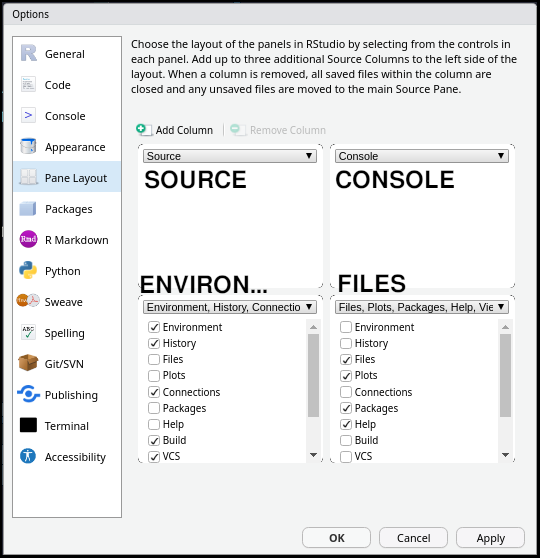
\includegraphics{./assets/rstudio-pane-layout.png}

}

\caption{Rstudio Global Options Pane Layout accessible by Tools}

\end{figure}

\hypertarget{recommended}{%
\section{Recommended}\label{recommended}}

I have two recommendations. Incorporate a project oriented workflow and
use version control.

\hypertarget{project-oriented-workflow}{%
\subsection{Project Oriented Workflow}\label{project-oriented-workflow}}

A project oriented workflow is a data analysis procedure that exists
within a container. Jennifer Bryan (citation needed) makes a strong case
for incorporating a project oriented workflow into your data analysis
system:

\begin{quote}
I suggest organizing each data analysis into a project: a folder on your
computer that holds all the files relevant to that particular piece of
work. I'm not assuming this is an RStudio Project, though this is a nice
implementation discussed below.

Any resident R script is written assuming that it will be run from a
fresh R process with working directory set to the project directory. It
creates everything it needs, in its own workspace or folder, and it
touches nothing it did not create. For example, it does not install
additional packages (another pet peeve of mine).

This convention guarantees that the project can be moved around on your
computer or onto other computers and will still ``just work''. I argue
that this is the only practical convention that creates reliable, polite
behavior across different computers or users and over time. This
convention is neither new, nor unique to R.

It's like agreeing that we will all drive on the left or the right. A
hallmark of civilization is following conventions that constrain your
behavior a little, in the name of public safety.
\end{quote}

An easy way to do this in RStudio is to create a new project for each
data analysis and use the \href{https://here.r-lib.org/}{\textbf{here}
package}. In my case, I have a folder
\texttt{\textasciitilde{}/projects/} where all my data analysis projects
live. If I have a data analysis project to summarize This makes it easy
for me to find the data, R scripts, or reports that I need.

\hypertarget{version-control}{%
\subsection{Version Control}\label{version-control}}

Version control allows for tracking changes to your project and makes it
easier for collaborating on projects. As described by Jennifer Bryan
(citation needed) in the \emph{Happy Git and GitHub for the useR} guide:

\begin{quote}
Git is a version control system. Its original purpose was to help groups
of developers work collaboratively on big software projects. Git manages
the evolution of a set of files -- called a repository -- in a sane,
highly structured way. If you have no idea what I'm talking about, think
of it as the ``Track Changes'' features from Microsoft Word on steroids.

Git has been re-purposed by the data science community. In addition to
using it for source code, we use it to manage the motley collection of
files that make up typical data analytical projects, which often consist
of data, figures, reports, and, yes, source code.
\end{quote}

Learning version about version control is beyond the scope of this
guide, but I recommend that you review the resource,
\href{https://happygitwithr.com/index.html}{Happy Git and GitHub for the
useR} by Jennifer Bryan.

\bookmarksetup{startatroot}

\hypertarget{project-oriented-workflow-1}{%
\chapter{Project Oriented Workflow}\label{project-oriented-workflow-1}}

\hypertarget{learning-objectives-2}{%
\section{Learning Objectives}\label{learning-objectives-2}}

In this chapter, readers will:

\begin{itemize}
\tightlist
\item
  identify the benefits of using RStudio projects
\end{itemize}

\hypertarget{introduction-2}{%
\section{Introduction}\label{introduction-2}}

RStudio projects make it easy to organize your data analysis in
self-contained projects. Refer to this page,
\href{https://support.rstudio.com/hc/en-us/articles/200526207-Using-Projects}{\emph{Using
RStudio Projects}} to learn more about RStudio projects. When I initiate
a new data analysis project I ground myself within the
\href{https://r4ds.had.co.nz/index.html}{R for Data Science} model:

\begin{figure}

{\centering 

\href{https://r4ds.had.co.nz/explore-intro.html}{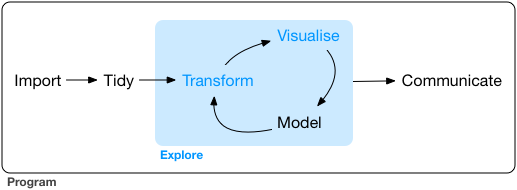
\includegraphics{./assets/data-science-explore.png}}

}

\caption{data exploration workflow program}

\end{figure}

To return to the project and make updates or run reports I open the
project in RStudio. This is much easier than fiddling with a working
directory.

\hypertarget{project-folder-structure}{%
\section{Project Folder Structure}\label{project-folder-structure}}

There is no right or wrong way to organize your data analysis. If you do
an internet search you will find many different strategies. This is the
approach I usually follow. I give my project a name and I make four
directories (folders):

\begin{verbatim}
project-name
    - data-tidy
    - data-raw
    - reports
    - scripts
\end{verbatim}

\hypertarget{data-tidy}{%
\subsection{data-tidy}\label{data-tidy}}

In this folder, I keep data that has already been processed. The files
in this sub-folder are ready for analysis.

\hypertarget{data-raw}{%
\subsection{data-raw}\label{data-raw}}

I do not make any changes to raw data. The data stays in the state I
received it. After I import data into my data analysis project and tidy
it, I save a copy in the \texttt{data-tidy} folder.

\hypertarget{reports}{%
\subsection{reports}\label{reports}}

This folder contains RMarkdown (or Quarto) reports. Learn about
RMarkdown by reviewing the documentation:
\url{https://rmarkdown.rstudio.com/}

\hypertarget{scripts}{%
\subsection{scripts}\label{scripts}}

I save my R scripts in this folder. Each script is intended to handle a
single task. My \texttt{import} script is only intended to read the
data. My \texttt{tidy} script is only intended to wrangle the data and
make it manageable. I usually name the scripts something like:

\begin{verbatim}
- 00-setup.R
- 01-import.R
- 02-tidy-and-transform.R
- 03-analysis.R
- 04-data-viz.R
\end{verbatim}

\bookmarksetup{startatroot}

\hypertarget{r-1}{%
\chapter{R}\label{r-1}}

\hypertarget{learning-objectives-3}{%
\section{Learning Objectives}\label{learning-objectives-3}}

In this chapter, readers will:

\begin{itemize}
\tightlist
\item
  identify the types of vectors and objects used in R
\item
  be able to assign a value to a named object
\item
  list the commands used to install and load packages
\end{itemize}

\hypertarget{introduction-3}{%
\section{Introduction}\label{introduction-3}}

In this section, we will review R. R is a powerful data science
statistical programming language. The
\href{https://cloud.r-project.org/doc/manuals/r-release/R-intro.html}{R
user manual} is a useful reference.

\hypertarget{r-is-a-calculator}{%
\section{R is a Calculator}\label{r-is-a-calculator}}

R can be used as an advanced scientific calculator. For example, say I
wanted to sum two values:

\begin{Shaded}
\begin{Highlighting}[]
\DecValTok{2}\SpecialCharTok{+}\DecValTok{2}
\end{Highlighting}
\end{Shaded}

\begin{verbatim}
[1] 4
\end{verbatim}

Or if I wanted to take the average of a set of values:

\begin{Shaded}
\begin{Highlighting}[]
\FunctionTok{mean}\NormalTok{(}\FunctionTok{c}\NormalTok{(}\DecValTok{2}\NormalTok{,}\DecValTok{4}\NormalTok{,}\DecValTok{6}\NormalTok{,}\DecValTok{8}\NormalTok{))}
\end{Highlighting}
\end{Shaded}

\begin{verbatim}
[1] 5
\end{verbatim}

Notice that I enclosed the values in \texttt{c()}. I used \texttt{c()}
to create a vector of my numeric values, and then I took a mean of those
values. I could instead assign (\texttt{\textless{}-}) the vector to a
named object:

\begin{Shaded}
\begin{Highlighting}[]
\NormalTok{my\_vector }\OtherTok{\textless{}{-}} \FunctionTok{c}\NormalTok{(}\DecValTok{2}\NormalTok{,}\DecValTok{4}\NormalTok{,}\DecValTok{6}\NormalTok{,}\DecValTok{8}\NormalTok{)}
\NormalTok{my\_vector}
\end{Highlighting}
\end{Shaded}

\begin{verbatim}
[1] 2 4 6 8
\end{verbatim}

\begin{Shaded}
\begin{Highlighting}[]
\FunctionTok{mean}\NormalTok{(my\_vector)}
\end{Highlighting}
\end{Shaded}

\begin{verbatim}
[1] 5
\end{verbatim}

Now each time I use \texttt{my\_vector}, R will know I mean
\texttt{2,4,6,8}.

\hypertarget{vectors}{%
\subsection{Vectors}\label{vectors}}

There are different types of vectors.

\begin{itemize}
\tightlist
\item
  numeric: numbers, like the example above
\item
  character: Character strings are entered using either matching double
  (``) or single (') quotes, but are printed using double quotes (or
  sometimes without quotes).
\item
  logical: The elements of a logical vector can have the values TRUE,
  FALSE, and NA (for ``not available'').
\end{itemize}

\hypertarget{other-types-of-objects}{%
\subsubsection{Other Types of Objects}\label{other-types-of-objects}}

And other objects exist:

\begin{itemize}
\tightlist
\item
  \emph{matrices} or more generally arrays are multi-dimensional
  generalizations of vectors. In fact, they are vectors that can be
  indexed by two or more indices and will be printed in special ways.
  See
  \href{https://cloud.r-project.org/doc/manuals/r-release/R-intro.html\#Arrays-and-matrices}{Arrays
  and matrices}.
\item
  \emph{factors} provide compact ways to handle categorical data. See
  \href{https://cloud.r-project.org/doc/manuals/r-release/R-intro.html\#Factors}{Ordered
  and unordered factors}.
\item
  \emph{lists} are a general form of vector in which the various
  elements need not be of the same type, and are often themselves
  vectors or lists. Lists provide a convenient way to return the results
  of a statistical computation. See
  \href{https://cloud.r-project.org/doc/manuals/r-release/R-intro.html\#Lists}{Lists}.
\item
  \emph{data frames} are matrix-like structures, in which the columns
  can be of different types. Think of data frames as `data matrices'
  with one row per observational unit but with (possibly) both numerical
  and categorical variables. Many experiments are best described by data
  frames: the treatments are categorical but the response is numeric.
  See
  \href{https://cloud.r-project.org/doc/manuals/r-release/R-intro.html\#Data-frames}{Data
  frames}.
\item
  \emph{functions} are themselves objects in R which can be stored in
  the project's workspace. This provides a simple and convenient way to
  extend R. See
  \href{https://cloud.r-project.org/doc/manuals/r-release/R-intro.html\#Writing-your-own-functions}{Writing
  your own functions}.
\end{itemize}

\hypertarget{use-r-for-formulas}{%
\subsection{Use R for Formulas}\label{use-r-for-formulas}}

For example, say we had a data set of observations of heights and
weights, and for some reason we wanted to calculate the BMI for each
observation. To get the mean for each observation I could do the
following:

\begin{Shaded}
\begin{Highlighting}[]
\FunctionTok{library}\NormalTok{(tidyverse) }\CommentTok{\# load the tidyverse package to use the pipe \%\textgreater{}\%}
\end{Highlighting}
\end{Shaded}

\begin{verbatim}
-- Attaching packages --------------------------------------- tidyverse 1.3.2 --
v ggplot2 3.3.6      v purrr   0.3.4 
v tibble  3.1.7      v dplyr   1.0.10
v tidyr   1.2.0      v stringr 1.4.1 
v readr   2.1.2      v forcats 0.5.2 
-- Conflicts ------------------------------------------ tidyverse_conflicts() --
x dplyr::filter() masks stats::filter()
x dplyr::lag()    masks stats::lag()
\end{verbatim}

\begin{Shaded}
\begin{Highlighting}[]
\FunctionTok{library}\NormalTok{(datasets) }\CommentTok{\# load the women dataset}

\NormalTok{women }\SpecialCharTok{\%\textgreater{}\%} \CommentTok{\# call the data set}
  \FunctionTok{mutate}\NormalTok{( }\CommentTok{\# create new variables for the data set I just called}
    \AttributeTok{bmi =}\NormalTok{ (weight }\SpecialCharTok{/}\NormalTok{ (height)}\SpecialCharTok{\^{}}\DecValTok{2}\NormalTok{)}\SpecialCharTok{*}\DecValTok{703} \CommentTok{\# new variable BMI using the formula for calculating BMI from weight in pounds and height in inches}
\NormalTok{  ) }\SpecialCharTok{\%\textgreater{}\%}
  \FunctionTok{head}\NormalTok{() }\CommentTok{\# limit my output to the first six observations}
\end{Highlighting}
\end{Shaded}

\begin{verbatim}
  height weight      bmi
1     58    115 24.03240
2     59    117 23.62856
3     60    120 23.43333
4     61    123 23.23811
5     62    126 23.04318
6     63    129 22.84883
\end{verbatim}

And if I wanted to get the mean or median of my sample's BMI, then I
could do this:

\begin{Shaded}
\begin{Highlighting}[]
\NormalTok{women }\SpecialCharTok{\%\textgreater{}\%} \CommentTok{\# call the dataset}
  \FunctionTok{mutate}\NormalTok{( }\CommentTok{\# create new variables}
    \AttributeTok{bmi =}\NormalTok{ (weight }\SpecialCharTok{/}\NormalTok{ (height)}\SpecialCharTok{\^{}}\DecValTok{2}\NormalTok{)}\SpecialCharTok{*}\DecValTok{703} \CommentTok{\# new variable BMI using the formula for calculating BMI from weight in pounds and height in inches}
\NormalTok{  ) }\SpecialCharTok{\%\textgreater{}\%}
  \FunctionTok{summarise}\NormalTok{( }\CommentTok{\# creates a new data frame}
    \CommentTok{\# It will contain one column for each grouping variable and one column for each of the summary statistics that you have specified}
    \AttributeTok{bmi\_mean =} \FunctionTok{mean}\NormalTok{(bmi), }\CommentTok{\# new variable}
    \AttributeTok{bmi\_median =} \FunctionTok{median}\NormalTok{(bmi) }\CommentTok{\# new variable}
\NormalTok{  )}
\end{Highlighting}
\end{Shaded}

\begin{verbatim}
  bmi_mean bmi_median
1 22.72443   22.46272
\end{verbatim}

\hypertarget{packages}{%
\section{Packages}\label{packages}}

Packages are bundles of code that add new functionality. This is a list
of the packages I recommend:

\begin{itemize}
\tightlist
\item
  \href{https://here.r-lib.org/}{here}: project oriented workflow
\item
  \href{https://www.tidyverse.org/}{tidyverse}: an opinionated
  collection of R packages designed for data science
\item
  \href{https://sfirke.github.io/janitor/}{janitor}: simple functions
  for examining and cleaning dirty data
\item
  \href{https://haven.tidyverse.org/}{haven}: enables R to read and
  write various data formats used by other statistical packages
  (i.e.~SAS)
\item
  \href{https://readxl.tidyverse.org/}{readxl}: makes it easy to get
  data out of Excel and into R
\item
  \href{https://lubridate.tidyverse.org/}{lubridate}: makes it easier to
  do the things R does with date-times and possible to do the things R
  does not
\item
  \href{https://rmarkdown.rstudio.com/lesson-1.html}{rmarkdown}: Turn
  your analyses into high quality documents, reports, presentations and
  dashboards
\item
  \href{https://yihui.org/knitr/}{knitr}: designed to be a transparent
  engine for dynamic report generation with R
\item
  \href{https://gt.rstudio.com/}{gt}: make wonderful-looking tables
  using the R programming language
\item
  \href{https://github.com/trinker/pacman}{pacman}: your new package
  manager
\item
  \href{https://docs.ropensci.org/qualtRics/}{qualtRics}: implements the
  retrieval of survey data using the Qualtrics API and aims to reduce
  the pre-processing steps needed in analyzing such surveys
\item
  \href{https://walker-data.com/tidycensus/}{tidycensus}: allows users
  to interface with a select number of the US Census Bureau's data APIs
  and return tidyverse-ready data frames, optionally with simple feature
  geometry included
\item
  \href{https://pkgs.rstudio.com/flexdashboard/}{flexdashboard}: make it
  easy to create interactive dashboards for R, using R Markdown
\item
  \href{https://pins.rstudio.com/}{pins}: publishes data, models, and
  other R objects, making it easy to share them across projects and with
  your colleagues
\item
  \href{https://cdcgov.github.io/Rnssp/}{Rnssp}: catalog of data
  processing and analytics tools, templates, and functions commonly used
  across the National Syndromic Surveillance Program at the Centers for
  Disease Control and Prevention (CDC)
\end{itemize}

\hypertarget{installing-packages}{%
\subsection{Installing Packages}\label{installing-packages}}

Install packages individually with
\texttt{install.packages("package-name")} or use
\texttt{pacman::p\_load(package-name)}.

This is \href{https://gist.github.com/stevenworthington/3178163}{R code}
that you can use to install the packages I listed above:

\begin{verbatim}
ipak <- function(pkg){
    new.pkg <- pkg[!(pkg %in% installed.packages()[, "Package"])]
    if (length(new.pkg)) 
        install.packages(new.pkg, dependencies = TRUE)
    sapply(pkg, require, character.only = TRUE)
}

# usage
packages <- c(
  "here",
  "tidyverse",
  "janitor",
  "haven",
  "readxl",
  "lubridate",
  "rmarkdown",
  "knitr",
  "gt",
  "pacman",
  "qualtRics",
  "tidycensus",
  "flexdashboard",
  "pins",
  "Rnssp"
)

ipak(packages)
\end{verbatim}

\hypertarget{loading-packages}{%
\subsection{Loading Packages}\label{loading-packages}}

Load packages for use with \texttt{library(package-name)} or
\texttt{pacman::p\_load(package-name)}.

\hypertarget{r-programming-tutorial---learn-the-basics-of-statistical-computing}{%
\section{R Programming Tutorial - Learn the Basics of Statistical
Computing}\label{r-programming-tutorial---learn-the-basics-of-statistical-computing}}

This is the Free Code Camp R Programming Tutorial (2019:
\url{https://www.youtube.com/watch?v=_V8eKsto3Ug}

\bookmarksetup{startatroot}

\hypertarget{import-data}{%
\chapter{Import Data}\label{import-data}}

\hypertarget{learning-objectives-4}{%
\section{Learning Objectives}\label{learning-objectives-4}}

In this chapter, readers will:

\begin{itemize}
\tightlist
\item
  identify how to import data from csv, xlsx, and sas7bdat files
\item
  identify how \texttt{janitor::clean\_names()} can make messy data,
  more neat
\end{itemize}

\hypertarget{introduction-4}{%
\section{Introduction}\label{introduction-4}}

Common file types to import may be one of:

\begin{itemize}
\tightlist
\item
  csv: comma separated value, a text file
\item
  xlsx: a Microsoft Excel workbook or worksheet
\item
  sas7bdat: SAS files
\end{itemize}

\hypertarget{csv}{%
\section{CSV}\label{csv}}

The \texttt{readr} package, loaded automatically with
\texttt{library(tidyverse)}, is the package used to read and import csv
files. Once loaded, the command to import a csv file is
\texttt{read\_csv("name-of-csv-file.csv")}. If we were interested in
\href{https://data.cdc.gov/Public-Health-Surveillance/United-States-COVID-19-Community-Levels-by-County/3nnm-4jni/data}{United
States COVID-19 Community Levels by County}, and we had downloaded data
in a csv file, we could import it by:

\begin{Shaded}
\begin{Highlighting}[]
\FunctionTok{library}\NormalTok{(tidyverse) }\CommentTok{\# load readr package from within tidyverse}
\end{Highlighting}
\end{Shaded}

\begin{verbatim}
-- Attaching packages --------------------------------------- tidyverse 1.3.2 --
v ggplot2 3.3.6      v purrr   0.3.4 
v tibble  3.1.7      v dplyr   1.0.10
v tidyr   1.2.0      v stringr 1.4.1 
v readr   2.1.2      v forcats 0.5.2 
-- Conflicts ------------------------------------------ tidyverse_conflicts() --
x dplyr::filter() masks stats::filter()
x dplyr::lag()    masks stats::lag()
\end{verbatim}

\begin{Shaded}
\begin{Highlighting}[]
\FunctionTok{library}\NormalTok{(janitor) }\CommentTok{\# load janitor package}
\end{Highlighting}
\end{Shaded}

\begin{verbatim}

Attaching package: 'janitor'

The following objects are masked from 'package:stats':

    chisq.test, fisher.test
\end{verbatim}

\begin{Shaded}
\begin{Highlighting}[]
\NormalTok{my\_csv\_data }\OtherTok{\textless{}{-}} \FunctionTok{read\_csv}\NormalTok{( }\CommentTok{\# assign the csv file to a new object}
  \AttributeTok{file =} \StringTok{"data{-}raw/us{-}covid{-}19{-}community{-}level{-}by{-}county.csv"} \CommentTok{\# this is the file to read}
\NormalTok{) }\SpecialCharTok{\%\textgreater{}\%}
  \FunctionTok{clean\_names}\NormalTok{() }\CommentTok{\# clean up the variable names}
\end{Highlighting}
\end{Shaded}

\begin{verbatim}
Rows: 1000 Columns: 12
-- Column specification --------------------------------------------------------
Delimiter: ","
chr  (5): county, county_fips, state, health_service_area, covid_19_communit...
dbl  (6): county_population, health_service_area_number, health_service_area...
dttm (1): date_updated

i Use `spec()` to retrieve the full column specification for this data.
i Specify the column types or set `show_col_types = FALSE` to quiet this message.
\end{verbatim}

\begin{Shaded}
\begin{Highlighting}[]
\FunctionTok{glimpse}\NormalTok{(my\_csv\_data) }\CommentTok{\# get a glimpse of the data }
\end{Highlighting}
\end{Shaded}

\begin{verbatim}
Rows: 1,000
Columns: 12
$ county                             <chr> "Wilcox County", "Caldwell County",~
$ county_fips                        <chr> "13315", "29025", "27111", "40021",~
$ state                              <chr> "Georgia", "Missouri", "Minnesota",~
$ county_population                  <dbl> 8635, 9020, 58746, 48657, 19169, 39~
$ health_service_area_number         <dbl> 197, 548, 582, 445, 316, 904, 435, ~
$ health_service_area                <chr> "Sumter, GA - Crisp, GA", "Jackson ~
$ health_service_area_population     <dbl> 86868, 1310630, 64718, 239733, 1626~
$ covid_inpatient_bed_utilization    <dbl> 0.2, 3.2, 6.3, 3.0, 5.8, 3.6, 1.1, ~
$ covid_hospital_admissions_per_100k <dbl> 2.3, 10.8, 12.4, 1.7, 18.4, 8.4, 8.~
$ covid_cases_per_100k               <dbl> 11.58, 277.16, 156.61, 2.06, 459.07~
$ covid_19_community_level           <chr> "Low", "High", "Medium", "Low", "Hi~
$ date_updated                       <dttm> 2022-05-19 07:00:00, 2022-06-23 07~
\end{verbatim}

\hypertarget{excel}{%
\section{Excel}\label{excel}}

The \texttt{readxl} package, loaded with \texttt{library(readxl)}, is
the package used to read and import xls and xlsx files. Once loaded, the
command to import an Excel worksheet is
\texttt{read\_excel("name-of-excel-file.xlsx")}. For example:

\begin{Shaded}
\begin{Highlighting}[]
\FunctionTok{library}\NormalTok{(tidyverse) }\CommentTok{\# load tidyverse package}
\FunctionTok{library}\NormalTok{(readxl) }\CommentTok{\# load readxl package}
\FunctionTok{library}\NormalTok{(janitor) }\CommentTok{\# load janitor package}

\NormalTok{my\_excel\_data }\OtherTok{\textless{}{-}} \FunctionTok{read\_excel}\NormalTok{( }\CommentTok{\# assign the excel file to a new object}
  \StringTok{"data{-}raw/us{-}covid{-}19{-}community{-}level{-}by{-}county.xlsx"} \CommentTok{\# name of excel file}
\NormalTok{) }\SpecialCharTok{\%\textgreater{}\%}
  \FunctionTok{clean\_names}\NormalTok{() }\CommentTok{\# clean up the variable names}

\FunctionTok{glimpse}\NormalTok{(my\_excel\_data) }\CommentTok{\# get a glimpse of the data}
\end{Highlighting}
\end{Shaded}

\begin{verbatim}
Rows: 1,000
Columns: 12
$ county                             <chr> "Wibaux County", "Blue Earth County~
$ county_fips                        <chr> "30109", "27013", "48109", "37005",~
$ state                              <chr> "Montana", "Minnesota", "Texas", "N~
$ county_population                  <chr> "969", "67653", "2171", "11137", "5~
$ health_service_area_number         <chr> "767", "573", "415", "73", "152", "~
$ health_service_area                <chr> "Richland, MT - Dawson, MT", "Blue ~
$ health_service_area_population     <chr> "22049", "131436", "846464", "62825~
$ covid_inpatient_bed_utilization    <chr> "1.8", "2.8", "2.2", "3.5", "1.5", ~
$ covid_hospital_admissions_per_100k <chr> "9.1", "10.7", "5.6", "12.7", "0.5"~
$ covid_cases_per_100k               <chr> "0", "181.81", "46.06", "26.94", "1~
$ covid_19_community_level           <chr> "Low", "Medium", "Low", "Medium", "~
$ date_updated                       <dttm> 2022-06-23 07:00:00, 2022-06-09 07~
\end{verbatim}

\hypertarget{sas}{%
\section{SAS}\label{sas}}

The \texttt{haven} package, loaded with \texttt{library(haven)}, is the
package used to read and import SAS files. Once loaded, the command to
import a SAS data set is
\texttt{read\_sas("name-of-sas-file.sas7bdat")}. For example:

\begin{Shaded}
\begin{Highlighting}[]
\FunctionTok{library}\NormalTok{(tidyverse) }\CommentTok{\# load tidyverse package}
\FunctionTok{library}\NormalTok{(haven) }\CommentTok{\# load haven package}
\FunctionTok{library}\NormalTok{(janitor) }\CommentTok{\# load janitor package}

\NormalTok{my\_sas\_data }\OtherTok{\textless{}{-}} \FunctionTok{read\_sas}\NormalTok{( }\CommentTok{\# assign the sas file to a new object}
  \StringTok{"data{-}raw/us{-}covid{-}19{-}community{-}level{-}by{-}county.sas7bdat"} \CommentTok{\# name of sas file}
\NormalTok{) }\SpecialCharTok{\%\textgreater{}\%}
  \FunctionTok{clean\_names}\NormalTok{() }\CommentTok{\# clean up the variable names}

\FunctionTok{glimpse}\NormalTok{(my\_sas\_data)}
\end{Highlighting}
\end{Shaded}

\begin{verbatim}
Rows: 1,000
Columns: 12
$ county                          <chr> "McCulloch County", "McIntosh County",~
$ county_fips                     <chr> "48307", "40091", "54003", "29143", "0~
$ state                           <chr> "Texas", "Oklahoma", "West Virginia", ~
$ county_population               <chr> "7984", "19596", "119171", "17076", "1~
$ health_service_area_number      <chr> "426", "445", "25", "563", "407", "904~
$ health_service_area             <chr> "Tom Green (San Angelo), TX - Runnels,~
$ health_service_area_population  <chr> "162408", "239733", "433166", "310071"~
$ covid_inpatient_bed_utilization <chr> "1.1", "2.9", "2.2", "0.5", "1", "3.9"~
$ covid_hospital_adm_per_100k     <chr> "12.9", "5.8", "3.5", "1.6", "5.1", "8~
$ covid_cases_per_100k            <chr> "137.78", "56.13", "23.5", "11.71", "2~
$ covid_19_community_level        <chr> "Medium", "Low", "Low", "Low", "Low", ~
$ date_updated                    <dttm> 2022-06-23, 2022-06-23, 2022-04-14, 2~
\end{verbatim}

\hypertarget{about-the-data}{%
\section{About the Data}\label{about-the-data}}

I used the following code to download the data:

\begin{verbatim}
library(tidyverse)
library(RSocrata)
library(janitor)

covid19 <- read.socrata(url = "https://data.cdc.gov/resource/3nnm-4jni.json") %>%
  as_tibble() %>%
  clean_names()
\end{verbatim}

And I saved a sample of the data to each of the three file types we
discussed earlier in this section.

\bookmarksetup{startatroot}

\hypertarget{tidy-data}{%
\chapter{Tidy Data}\label{tidy-data}}

This page is still being worked on.

\hypertarget{learning-objectives-5}{%
\section{Learning Objectives}\label{learning-objectives-5}}

In this chapter, readers will:

\begin{itemize}
\tightlist
\item
  identify what makes data ``tidy''
\item
  identify how to make messy data tidy
\end{itemize}

\hypertarget{introduction-5}{%
\section{Introduction}\label{introduction-5}}

After importing my data, but before any meaningful data analysis, I make
sure my data is ``tidy''. Tidy data follows three rules as suggested by
\href{https://r4ds.had.co.nz/tidy-data.html}{Hadley Wickham and Garrett
Grolemund}:

\begin{enumerate}
\def\labelenumi{\arabic{enumi}.}
\tightlist
\item
  Each variable must have its own column.
\item
  Each observation must have its own row.
\item
  Each value must have its own cell.
\end{enumerate}

\begin{figure}

{\centering 

\href{https://r4ds.had.co.nz/tidy-data.html}{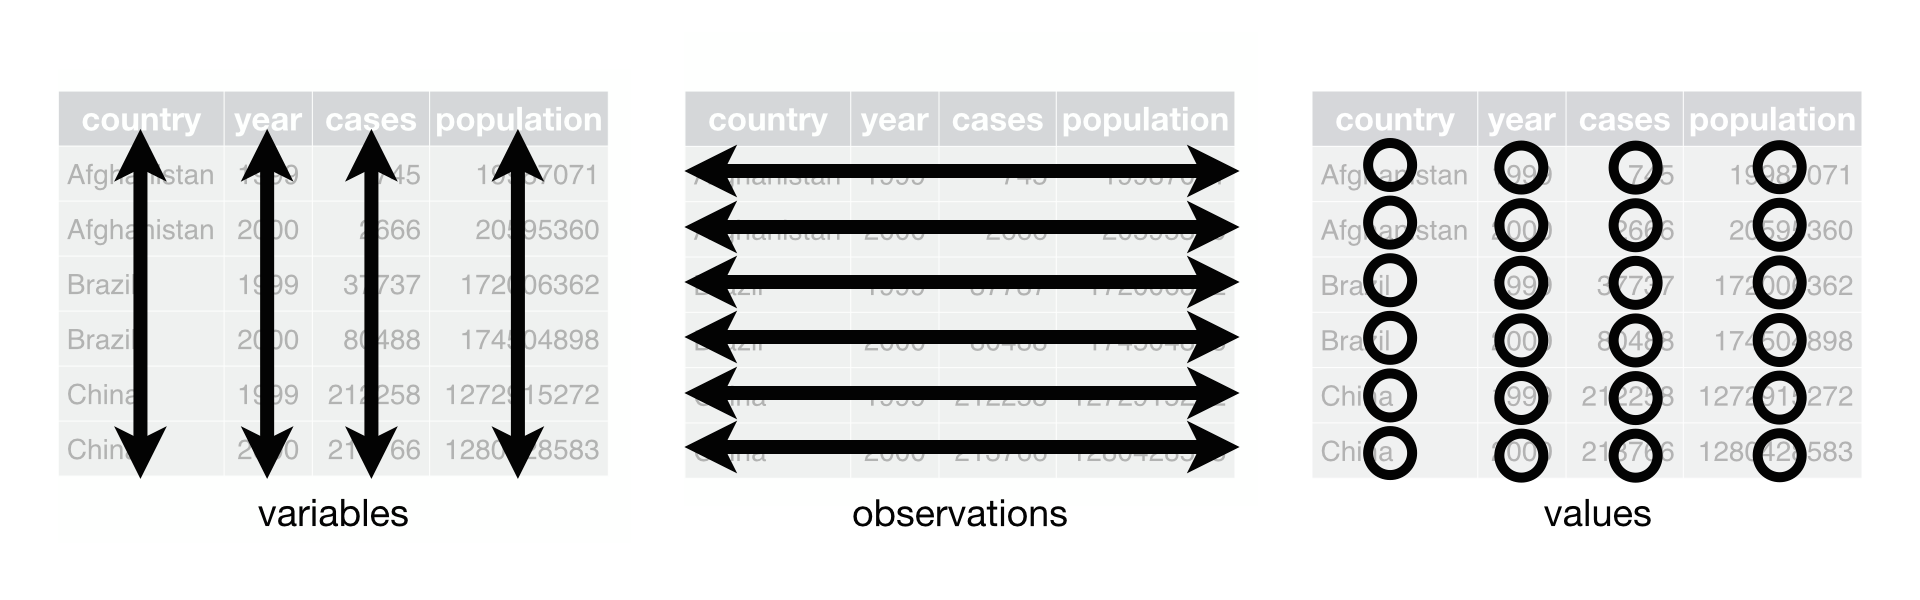
\includegraphics{./assets/tidy-1.png}}

}

\caption{rules of tidy data}

\end{figure}

\begin{Shaded}
\begin{Highlighting}[]
\FunctionTok{library}\NormalTok{(tidyverse) }\CommentTok{\# load readr package from within tidyverse}
\end{Highlighting}
\end{Shaded}

\begin{verbatim}
-- Attaching packages --------------------------------------- tidyverse 1.3.2 --
v ggplot2 3.3.6      v purrr   0.3.4 
v tibble  3.1.7      v dplyr   1.0.10
v tidyr   1.2.0      v stringr 1.4.1 
v readr   2.1.2      v forcats 0.5.2 
-- Conflicts ------------------------------------------ tidyverse_conflicts() --
x dplyr::filter() masks stats::filter()
x dplyr::lag()    masks stats::lag()
\end{verbatim}

\begin{Shaded}
\begin{Highlighting}[]
\FunctionTok{library}\NormalTok{(tidycensus) }\CommentTok{\# load the tidycensus package}
\FunctionTok{library}\NormalTok{(janitor) }\CommentTok{\# load janitor package}
\end{Highlighting}
\end{Shaded}

\begin{verbatim}

Attaching package: 'janitor'

The following objects are masked from 'package:stats':

    chisq.test, fisher.test
\end{verbatim}

\begin{Shaded}
\begin{Highlighting}[]
\CommentTok{\# import US Census ACS data using the tidycensus package library }
\NormalTok{poverty\_wide }\OtherTok{\textless{}{-}} \FunctionTok{get\_acs}\NormalTok{(}
  \AttributeTok{geography =} \StringTok{"tract"}\NormalTok{,}
  \AttributeTok{variables =} \FunctionTok{c}\NormalTok{(}
    \StringTok{"population"} \OtherTok{=} \StringTok{"S1701\_C01\_001"}\NormalTok{,}
    \StringTok{"poverty"} \OtherTok{=} \StringTok{"S1701\_C03\_002"}\NormalTok{,}
    \StringTok{"median\_income"} \OtherTok{=} \StringTok{"S1901\_C01\_012"}\NormalTok{,}
    \StringTok{"median\_rent"} \OtherTok{=} \StringTok{"DP04\_0134"}\NormalTok{,}
    \StringTok{"median\_age"} \OtherTok{=} \StringTok{"B01002\_001"}\NormalTok{,}
    \StringTok{"bachelor\_degree\_percent"} \OtherTok{=} \StringTok{"DP02\_0065P"}\NormalTok{,}
    \StringTok{"broadband\_percent"} \OtherTok{=} \StringTok{"DP02\_0153P"}\NormalTok{,}
    \StringTok{"hispanic\_percent"} \OtherTok{=} \StringTok{"DP05\_0071P"}\NormalTok{,}
    \StringTok{"sex\_percent"} \OtherTok{=} \StringTok{"S0101\_C06\_008"}\NormalTok{,}
    \StringTok{"womens\_earnings\_percent"} \OtherTok{=} \StringTok{"S2411\_C04\_001"}\NormalTok{,}
    \StringTok{"gini\_index"} \OtherTok{=} \StringTok{"B19083\_001"}\NormalTok{,}
    \StringTok{"white\_not\_hispanic"} \OtherTok{=} \StringTok{"B01001H\_001"}
\NormalTok{    ),}
  \AttributeTok{year =} \DecValTok{2019}\NormalTok{,}
  \AttributeTok{geometry =} \ConstantTok{FALSE}\NormalTok{,}
  \AttributeTok{survey =} \StringTok{"acs5"}\NormalTok{,}
  \AttributeTok{state =} \StringTok{"AZ"}\NormalTok{,}
  \AttributeTok{cache\_table =} \ConstantTok{TRUE}\NormalTok{,}
  \AttributeTok{output =} \StringTok{"wide"}
\NormalTok{) }\SpecialCharTok{\%\textgreater{}\%}
  \FunctionTok{clean\_names}\NormalTok{() }\CommentTok{\# use janitor to clean the names }
\end{Highlighting}
\end{Shaded}

\begin{verbatim}
Getting data from the 2015-2019 5-year ACS
Fetching data by table type ("B/C", "S", "DP") and combining the result.
\end{verbatim}

\begin{Shaded}
\begin{Highlighting}[]
\CommentTok{\# inspect the dataset}
\CommentTok{\# note the data is wide}
\FunctionTok{glimpse}\NormalTok{(poverty\_wide)}
\end{Highlighting}
\end{Shaded}

\begin{verbatim}
Rows: 1,526
Columns: 26
$ geoid                     <chr> "04001942600", "04001942700", "04001944000",~
$ name                      <chr> "Census Tract 9426, Apache County, Arizona",~
$ median_age_e              <dbl> 32.8, 33.6, 33.9, 27.9, 27.9, 27.9, 34.2, 30~
$ median_age_m              <dbl> 4.5, 2.5, 3.5, 1.7, 5.9, 4.0, 2.2, 2.1, 1.9,~
$ gini_index_e              <dbl> 0.5612, 0.4984, 0.5446, 0.5359, 0.4998, 0.52~
$ gini_index_m              <dbl> 0.0521, 0.0208, 0.0378, 0.0263, 0.0444, 0.05~
$ white_not_hispanic_e      <dbl> 0, 35, 140, 154, 188, 17, 72, 81, 48, 113, 7~
$ white_not_hispanic_m      <dbl> 12, 25, 61, 53, 74, 20, 30, 80, 29, 62, 46, ~
$ population_e              <dbl> 1742, 5345, 6543, 5639, 4400, 4009, 6005, 39~
$ population_m              <dbl> 206, 365, 570, 461, 449, 664, 378, 342, 272,~
$ poverty_e                 <dbl> 45.4, 44.7, 57.5, 61.7, 62.2, 60.6, 53.6, 45~
$ poverty_m                 <dbl> 13.4, 7.0, 9.6, 6.6, 12.7, 14.6, 8.1, 8.2, 7~
$ median_income_e           <dbl> 19250, 26646, 33472, 24696, 26840, 24173, 20~
$ median_income_m           <dbl> 3355, 2332, 8117, 3776, 5187, 4876, 1680, 43~
$ sex_percent_e             <dbl> 4.6, 6.8, 6.7, 3.9, 2.7, 6.0, 6.0, 3.9, 7.0,~
$ sex_percent_m             <dbl> 2.5, 1.8, 1.8, 1.2, 1.9, 3.0, 2.0, 1.4, 1.8,~
$ womens_earnings_percent_e <dbl> 137.3, 87.1, 114.1, 97.8, 88.8, 84.9, 94.7, ~
$ womens_earnings_percent_m <dbl> 56.8, 10.8, 41.4, 14.2, 69.8, 48.6, 12.0, 18~
$ median_rent_e             <dbl> NA, 579, 549, 339, 473, 537, 414, 426, 482, ~
$ median_rent_m             <dbl> NA, 104, 65, 42, 39, 142, 20, 41, 49, 62, 12~
$ bachelor_degree_percent_e <dbl> 2.1, 4.6, 6.2, 6.2, 6.4, 6.8, 4.5, 6.7, 5.7,~
$ bachelor_degree_percent_m <dbl> 1.2, 1.0, 2.3, 1.6, 2.8, 3.5, 1.2, 1.4, 1.4,~
$ broadband_percent_e       <dbl> 12.1, 17.8, 29.9, 26.2, 16.9, 16.0, 10.8, 27~
$ broadband_percent_m       <dbl> 4.9, 2.7, 4.9, 3.6, 5.4, 6.2, 2.2, 3.9, 3.2,~
$ hispanic_percent_e        <dbl> 0.0, 0.6, 1.1, 1.6, 0.3, 0.1, 0.7, 0.8, 2.6,~
$ hispanic_percent_m        <dbl> 2.0, 0.5, 0.9, 0.8, 0.5, 0.3, 0.6, 0.8, 1.2,~
\end{verbatim}

\begin{Shaded}
\begin{Highlighting}[]
\CommentTok{\# use pivot\_longer to make the data tidy }
\NormalTok{poverty\_wide }\SpecialCharTok{\%\textgreater{}\%}
  \FunctionTok{pivot\_longer}\NormalTok{(}
    \AttributeTok{cols =} \FunctionTok{all\_of}\NormalTok{(}\FunctionTok{c}\NormalTok{(}\StringTok{"geoid"}\NormalTok{, }\StringTok{"name"}\NormalTok{)),}
    \AttributeTok{names\_to =} \StringTok{"name"}\NormalTok{,}
    \AttributeTok{values\_to =} \StringTok{"value"}
\NormalTok{  )}
\end{Highlighting}
\end{Shaded}

\begin{verbatim}
# A tibble: 3,052 x 26
   median_age_e median~1 gini_~2 gini_~3 white~4 white~5 popul~6 popul~7 pover~8
          <dbl>    <dbl>   <dbl>   <dbl>   <dbl>   <dbl>   <dbl>   <dbl>   <dbl>
 1         32.8      4.5   0.561  0.0521       0      12    1742     206    45.4
 2         32.8      4.5   0.561  0.0521       0      12    1742     206    45.4
 3         33.6      2.5   0.498  0.0208      35      25    5345     365    44.7
 4         33.6      2.5   0.498  0.0208      35      25    5345     365    44.7
 5         33.9      3.5   0.545  0.0378     140      61    6543     570    57.5
 6         33.9      3.5   0.545  0.0378     140      61    6543     570    57.5
 7         27.9      1.7   0.536  0.0263     154      53    5639     461    61.7
 8         27.9      1.7   0.536  0.0263     154      53    5639     461    61.7
 9         27.9      5.9   0.500  0.0444     188      74    4400     449    62.2
10         27.9      5.9   0.500  0.0444     188      74    4400     449    62.2
# ... with 3,042 more rows, 17 more variables: poverty_m <dbl>,
#   median_income_e <dbl>, median_income_m <dbl>, sex_percent_e <dbl>,
#   sex_percent_m <dbl>, womens_earnings_percent_e <dbl>,
#   womens_earnings_percent_m <dbl>, median_rent_e <dbl>, median_rent_m <dbl>,
#   bachelor_degree_percent_e <dbl>, bachelor_degree_percent_m <dbl>,
#   broadband_percent_e <dbl>, broadband_percent_m <dbl>,
#   hispanic_percent_e <dbl>, hispanic_percent_m <dbl>, name <chr>, ...
\end{verbatim}

\begin{Shaded}
\begin{Highlighting}[]
\NormalTok{poverty\_tidy }\OtherTok{\textless{}{-}} \FunctionTok{get\_acs}\NormalTok{(}
  \AttributeTok{geography =} \StringTok{"tract"}\NormalTok{,}
  \AttributeTok{variables =} \FunctionTok{c}\NormalTok{(}
    \StringTok{"population"} \OtherTok{=} \StringTok{"S1701\_C01\_001"}\NormalTok{,}
    \StringTok{"poverty"} \OtherTok{=} \StringTok{"S1701\_C03\_002"}\NormalTok{,}
    \StringTok{"median\_income"} \OtherTok{=} \StringTok{"S1901\_C01\_012"}\NormalTok{,}
    \StringTok{"median\_rent"} \OtherTok{=} \StringTok{"DP04\_0134"}\NormalTok{,}
    \StringTok{"median\_age"} \OtherTok{=} \StringTok{"B01002\_001"}\NormalTok{,}
    \StringTok{"bachelor\_degree\_percent"} \OtherTok{=} \StringTok{"DP02\_0065P"}\NormalTok{,}
    \StringTok{"broadband\_percent"} \OtherTok{=} \StringTok{"DP02\_0153P"}\NormalTok{,}
    \StringTok{"hispanic\_percent"} \OtherTok{=} \StringTok{"DP05\_0071P"}\NormalTok{,}
    \StringTok{"sex\_percent"} \OtherTok{=} \StringTok{"S0101\_C06\_008"}\NormalTok{,}
    \StringTok{"womens\_earnings\_percent"} \OtherTok{=} \StringTok{"S2411\_C04\_001"}\NormalTok{,}
    \StringTok{"gini\_index"} \OtherTok{=} \StringTok{"B19083\_001"}\NormalTok{,}
    \StringTok{"white\_not\_hispanic"} \OtherTok{=} \StringTok{"B01001H\_001"}
\NormalTok{    ),}
  \AttributeTok{year =} \DecValTok{2019}\NormalTok{,}
  \AttributeTok{geometry =} \ConstantTok{FALSE}\NormalTok{,}
  \AttributeTok{survey =} \StringTok{"acs5"}\NormalTok{,}
  \AttributeTok{state =} \StringTok{"AZ"}\NormalTok{,}
  \AttributeTok{cache\_table =} \ConstantTok{TRUE}\NormalTok{,}
  \AttributeTok{output =} \StringTok{"tidy"}
\NormalTok{) }\SpecialCharTok{\%\textgreater{}\%}
  \FunctionTok{clean\_names}\NormalTok{()}
\end{Highlighting}
\end{Shaded}

\begin{verbatim}
Getting data from the 2015-2019 5-year ACS
Fetching data by table type ("B/C", "S", "DP") and combining the result.
\end{verbatim}

\begin{Shaded}
\begin{Highlighting}[]
\FunctionTok{glimpse}\NormalTok{(poverty\_tidy)}
\end{Highlighting}
\end{Shaded}

\begin{verbatim}
Rows: 18,312
Columns: 5
$ geoid    <chr> "04001942600", "04001942600", "04001942600", "04001942600", "~
$ name     <chr> "Census Tract 9426, Apache County, Arizona", "Census Tract 94~
$ variable <chr> "white_not_hispanic", "median_age", "gini_index", "sex_percen~
$ estimate <dbl> 0.0000, 32.8000, 0.5612, 4.6000, 1742.0000, 45.4000, 19250.00~
$ moe      <dbl> 12.0000, 4.5000, 0.0521, 2.5000, 206.0000, 13.4000, 3355.0000~
\end{verbatim}

\bookmarksetup{startatroot}

\hypertarget{section}{%
\chapter{}\label{section}}

\bookmarksetup{startatroot}

\hypertarget{section-1}{%
\chapter{}\label{section-1}}

\bookmarksetup{startatroot}

\hypertarget{section-2}{%
\chapter{}\label{section-2}}

\bookmarksetup{startatroot}

\hypertarget{references}{%
\chapter*{References}\label{references}}
\addcontentsline{toc}{chapter}{References}

\hypertarget{refs}{}
\begin{CSLReferences}{0}{0}
\end{CSLReferences}



\end{document}
